\documentclass[
    headings=optiontotocandhead,% Erweiterung für das optionale Argument der
                                % Gliederungsbefehle aktiviert.
    twoside,
    numbers=noenddot,% Keine Punkte am Ende der Gliederungsnummern und davon
                     % abgeleiteten Nummern
    toc=flat, %Flache TOC
    12pt, % Schriftgröße
    titlepage, % es wird eine Titelseite verwendet
    parskip=full, % Abstand zwischen Absätzen (ganze Zeile)
    listof=totoc, % Verzeichnisse im Inhaltsverzeichnis aufführen
    listof=flat, % mehr Abstand für grosse Zahlen
    numbers=noenddot, % kein Punkt am Ende bei Nummern
    %%enlargefirstpage,% Gibt es bei scrartcl nicht!!!!
    bibliography=totoc, % Literaturverzeichnis im Inhaltsverzeichnis aufführen
    %index=totoc, % Index im Inhaltsverzeichnis aufführen
    %captions=tableheading, % Beschriftung von Tabellen für Ausgabe oberhalb
                           % der Tabelle formatieren
    %draft % Status des Dokuments (final/draft) draft hinzufügen zum anziegen
    %%der zeilen ende
    a4paper,DIV=14,
    BCOR=15mm,
    % captions=tablesignature,
]{scrbook}

\setcounter{secnumdepth}{3}

\usepackage{dirtree}
\usepackage{textcomp}

\usepackage[T1]{fontenc}
\usepackage[utf8]{inputenc}

\usepackage[english, ngerman, naustrian]{babel} % your native language must be the last one!!

\usepackage{lastpage}
\usepackage{listings}
\usepackage{blindtext}

%% Aufzählungen nicht so weit einrücken
\usepackage[inline]{enumitem}
%\setitemize{leftmargin=*}
% Listen etwas wenige einrücken, erfordert enumitem
\setitemize{leftmargin=*}

\usepackage{lmodern}

\usepackage{xspace}

\usepackage{graphicx}

\makeatletter
    \def\maxwidth{\ifdim\Gin@nat@width>\linewidth\linewidth\else\Gin@nat@width\fi}
    \def\maxheight{\ifdim\Gin@nat@height>\textheight\textheight\else\Gin@nat@height\fi}
\makeatother
% Scale images if necessary, so that they will not overflow the page
% margins by default, and it is still possible to overwrite the defaults
% using explicit options in \includegraphics[width, height, ...]{}
\setkeys{Gin}{width=\maxwidth,height=\maxheight,keepaspectratio}


%%? \usepackage{textcomp}
\usepackage[hyphens]{url}
\usepackage{makeidx}
\makeindex
%%? \usepackage{graphicx}
\usepackage[numbers]{natbib}
\PassOptionsToPackage{normalem}{ulem}
\usepackage{ulem}

\usepackage{needspace}

\setlength\partopsep{0.5ex}%schoenere Listen
\usepackage[bottom]{footmisc}%fussnote ganz unten

\usepackage[]{microtype}
\UseMicrotypeSet[protrusion]{basicmath} % disable protrusion for tt fonts

\usepackage{multirow}   % Allows table elements to span several rows.
\usepackage{booktabs}   % Improves the typesettings of tables.
\usepackage{subcaption} % Allows the use of subfigures and enables their referencing.
\usepackage[ruled,linesnumbered,algochapter]{algorithm2e} % Enables the writing of pseudo code.
\usepackage[usenames,dvipsnames,table]{xcolor} % Allows the definition and use of colors. This package has to be included before tikz.
\usepackage{nag}       % Issues warnings when best practices in writing LaTeX documents are violated.
\usepackage{todonotes} % Provides tooltip-like todo notes.

\usepackage{color}

%% bessere Suche im PDF
\input{glyphtounicode}
\pdfgentounicode=1
%%%%%%%%%%%%%%%%%%%%%%%%%%%%%%%%%%%%%%%%%%%%%%%%%%%%%%%%%%%%%%%%%%%%%%%%%%%%%%%%%%

%  Kopf und Fußzeilen -- links und rechts verschieden
\newcommand{\kopfseitenummer}{{\bfseries \thepage}}
\newcommand{\kopfkapl}{{\bfseries\leftmark}}
\newcommand{\kopfkapr}{{\bfseries\rightmark}}
\newcommand{\kopfbild}{\voffset7mm
\includegraphics[width=25mm]{HTL3RLogoRGB}}
\newcommand{\kopfHTL}{Höhere Technische Bundeslehranstalt Wien 3, \\Rennweg 	Abteilung für Informationstechnologie}

\usepackage[automark,headsepline,footsepline,plainfootsepline]{scrlayer-scrpage}
%\automark[chapter]{chapter}% Eventuell wenn doppelseitig
\setkomafont{pageheadfoot}{\normalcolor\footnotesize\scshape}
\setkomafont{pagenumber}{\normalfont\normalsize}
\clearpairofpagestyles
\ihead{\headmark}
\ohead{\kopfbild}
\ifoot{\kapitelautor}
\ofoot{\pagemark}
\ModifyLayer[addvoffset=-.6ex]{scrheadings.foot.above.line}% Linie verschieben
\ModifyLayer[addvoffset=-.6ex]{plain.scrheadings.foot.above.line}% Linie verschieben
\setlength{\headheight}{32pt}

% alle Seiten mit Kopfzeile
\renewcommand{\chapterpagestyle}{scrheadings}

%% Kapitel - aufwändige Kapitelüberschriften
%Options: Sonny, Lenny, Glenn, Conny, Rejne, Bjarne, Bjornstrup
%\usepackage[Bjornstrup]{fncychap}
% Alternative:
%\usepackage{titlesec}

% Verzeichnisse - aufwändiger
%\usepackage{tocloft}


%% Code Beispiele
%% eine Variante
\usepackage{listings}
\renewcommand{\lstlistingname}{\inputencoding{utf8}Listing}
%% andere Variante
%\usepackage{minted}
%\setminted{
%  linenos,
%  frame=lines,
%  framesep=2mm,
%  breaklines=true
%}
% Beispiel
%\begin{listing}[H]
%\begin{minted}{bash}
%...
%\end{minted}
%\caption{Beschreibung}
%\end{listing}
%% dritte Variante
% mit/für pandoc
% create
% pandoc -s sample.md -o sample.tex
% -> copy/paste

\usepackage{fancyvrb}
\newcommand{\VerbBar}{|}
\newcommand{\VERB}{\Verb[commandchars=\\\{\}]}
\DefineVerbatimEnvironment{Highlighting}{Verbatim}{commandchars=\\\{\}}
% Add ',fontsize=\small' for more characters per line
\newenvironment{Shaded}{}{}
\newcommand{\KeywordTok}[1]{\textcolor[rgb]{0.00,0.44,0.13}{\textbf{#1}}}
\newcommand{\DataTypeTok}[1]{\textcolor[rgb]{0.56,0.13,0.00}{#1}}
\newcommand{\DecValTok}[1]{\textcolor[rgb]{0.25,0.63,0.44}{#1}}
\newcommand{\BaseNTok}[1]{\textcolor[rgb]{0.25,0.63,0.44}{#1}}
\newcommand{\FloatTok}[1]{\textcolor[rgb]{0.25,0.63,0.44}{#1}}
\newcommand{\ConstantTok}[1]{\textcolor[rgb]{0.53,0.00,0.00}{#1}}
\newcommand{\CharTok}[1]{\textcolor[rgb]{0.25,0.44,0.63}{#1}}
\newcommand{\SpecialCharTok}[1]{\textcolor[rgb]{0.25,0.44,0.63}{#1}}
\newcommand{\StringTok}[1]{\textcolor[rgb]{0.25,0.44,0.63}{#1}}
\newcommand{\VerbatimStringTok}[1]{\textcolor[rgb]{0.25,0.44,0.63}{#1}}
\newcommand{\SpecialStringTok}[1]{\textcolor[rgb]{0.73,0.40,0.53}{#1}}
\newcommand{\ImportTok}[1]{#1}
\newcommand{\CommentTok}[1]{\textcolor[rgb]{0.38,0.63,0.69}{\textit{#1}}}
\newcommand{\DocumentationTok}[1]{\textcolor[rgb]{0.73,0.13,0.13}{\textit{#1}}}
\newcommand{\AnnotationTok}[1]{\textcolor[rgb]{0.38,0.63,0.69}{\textbf{\textit{#1}}}}
\newcommand{\CommentVarTok}[1]{\textcolor[rgb]{0.38,0.63,0.69}{\textbf{\textit{#1}}}}
\newcommand{\OtherTok}[1]{\textcolor[rgb]{0.00,0.44,0.13}{#1}}
\newcommand{\FunctionTok}[1]{\textcolor[rgb]{0.02,0.16,0.49}{#1}}
\newcommand{\VariableTok}[1]{\textcolor[rgb]{0.10,0.09,0.49}{#1}}
\newcommand{\ControlFlowTok}[1]{\textcolor[rgb]{0.00,0.44,0.13}{\textbf{#1}}}
\newcommand{\OperatorTok}[1]{\textcolor[rgb]{0.40,0.40,0.40}{#1}}
\newcommand{\BuiltInTok}[1]{#1}
\newcommand{\ExtensionTok}[1]{#1}
\newcommand{\PreprocessorTok}[1]{\textcolor[rgb]{0.74,0.48,0.00}{#1}}
\newcommand{\AttributeTok}[1]{\textcolor[rgb]{0.49,0.56,0.16}{#1}}
\newcommand{\RegionMarkerTok}[1]{#1}
\newcommand{\InformationTok}[1]{\textcolor[rgb]{0.38,0.63,0.69}{\textbf{\textit{#1}}}}
\newcommand{\WarningTok}[1]{\textcolor[rgb]{0.38,0.63,0.69}{\textbf{\textit{#1}}}}
\newcommand{\AlertTok}[1]{\textcolor[rgb]{1.00,0.00,0.00}{\textbf{#1}}}
\newcommand{\ErrorTok}[1]{\textcolor[rgb]{1.00,0.00,0.00}{\textbf{#1}}}
\newcommand{\NormalTok}[1]{#1}


%% should be last packages
\usepackage{scrhack}

\usepackage[unicode=true,
 bookmarks=true,bookmarksnumbered=false,bookmarksopen=false,
 breaklinks=true,pdfborder={0 0 0},backref=false,colorlinks=false]
 {hyperref}
\hypersetup{pdftitle={Diplomarbeit Titel},
 pdfauthor={Wer auch immer},
 pdfsubject={Diplomarbeit},
 pdfkeywords={dies, das}}
\urlstyle{same} % don't use monospace font for urls

%% for pandoc
\providecommand{\tightlist}{%
  \setlength{\itemsep}{0pt}\setlength{\parskip}{0pt}}

% Auch Fußnoten bündig ausrichten
\deffootnote[]{1em}{1em}{\textsuperscript{\thefootnotemark\ }}
%% setup
\sloppy % weniger Meldungen
\voffset7mm % etwas nach unten

%% schöner: 10000 -- gar keine, 1000 als Mittelweg
\clubpenalty = 1000 % Schusterjungen verhindern
\widowpenalty = 1000 % Hurenkinder verhindern
\displaywidowpenalty = 1000

%%%%%%%%%%%%%%%%%%%%%%%%%%%%%%%%%%%%%%%%%%%%%%%%%%%%%%%%%%%%%%%%%%%%%%%%%%%%%%%%%%
\begin{document}
%% wir schreiben keine Umlaut mit "a "o
\shorthandoff{"}
%% mit kapitelautor kann man den Autor festlegen oder auf leer setzen - steht dann in der Fußzeile.
\newcommand{\kapitelautor}{}

%%
\newcommand{\strong}[1]{\textbf{#1}}
\newcommand{\code}[1]{\texttt{#1}}

% einfaches "siehe ..." - das Ziel muss man markieren mit \label{name} -- macht pandoc automatisch
\newcommand{\kap}[1]{Kapitel~\ref{#1}, Seite~\pageref{#1}}
\newcommand{\siehe}[1]{siehe \kap{#1}}
\newcommand{\abb}[1]{Abbildung~\ref{#1}, Seite~\pageref{#1}}

%% http://ieg.ifs.tuwien.ac.at/~aigner/download/tuwien.sty
%Div. Abkürzungen (in Anlehnung an Jochen Köpper, jkthesis):
%\RequirePackage{xspace}
\newcommand{\bzw}{bzw.\@\xspace}
\newcommand{\bzgl}{bzgl.\@\xspace}
\newcommand{\ca}{ca.\@\xspace}
\newcommand{\dah}{d.\thinspace{}h.\@\xspace}
\newcommand{\Dah}{D.\thinspace{}h.\@\xspace}
\newcommand{\ds}{d.\thinspace{}s.\@\xspace}
\newcommand{\evtl}{evtl.\@\xspace}
\newcommand{\ua}{u.\thinspace{}a.\@\xspace}
\newcommand{\Ua}{U.\thinspace{}a.\@\xspace}
\newcommand{\usw}{usw.\@\xspace}
\newcommand{\va}{v.\thinspace{}a.\@\xspace}
\newcommand{\vgl}{vgl.\@\xspace}
\newcommand{\zB}{z.\thinspace{}B.\@\xspace}
\newcommand{\ZB}{Zum Beispiel\xspace} 

%% https://github.com/Digital-Media/HagenbergThesis
\newcommand{\latex}{La\-TeX\xspace} % kein schnoerkeliges LaTeX mehr
\newcommand{\tex}{TeX\xspace}       % kein schnoerkeliges TeX mehr
\newcommand{\bs}{\textbackslash}    % Backslash character
\newcommand{\obnh}{\hskip 0pt } %optional break without hyphen: e.g. PlugIn{\obnh}Filter

\newcommand{\sa}{s.\ auch\@\xspace}
\newcommand{\so}{s.\ oben\xspace}
\newcommand{\su}{s.\ unten\@\xspace}

\newcommand{\uae}{u.\thinspace{}\"A.\@\xspace}
\newcommand{\uva}{u.\thinspace{}v.\thinspace{}a.\@\xspace}
\newcommand{\uvm}{u.\thinspace{}v.\thinspace{}m.\@\xspace}



%%%%%Anfang Titelseite
%\pagenumbering{roman}
\frontmatter % Switches to roman numbering
\title{Diplomarbeit}
\begin{titlepage}
\begin{minipage}[b]{1\columnwidth}
\parbox[b]{50mm}{
\includegraphics[width=45mm]{HTL3RLogoRGB}}
\hfill
\parbox[b]{130mm}{\footnotesize \textsc{Höhere Technische Bundeslehranstalt} Wien 3, Rennweg\\
IT \& Mechatronik\\
\\
HTL Rennweg :: Rennweg 89b\\
A-1030 Wien :: Tel +43 1 24215-10 :: Fax DW 18
}\\
\mbox{}
\end{minipage}

\vspace{1cm}


\begin{center}
\textbf{\LARGE{}Diplomarbeit}{\large{}}\\
{\large{}\vspace{15mm}
 }\textbf{\large{}Mediatrix}\\
\textbf{\large{}Ausgeschriebener Titel der Diplomarbeit}\\
 \vspace{15mm}
 ausgeführt an der\\
 Höheren Abteilung für Informationstechnologie/Medientechnik\\
 der Höheren Technischen Lehranstalt Wien 3 Rennweg\\
 \vspace{1cm}
 im Schuljahr 2017/2018\\
 \vspace{1cm}
 durch\\
 \vspace{0.5cm}
\textbf{\large{}Nußbaumer Dominik}\\
\textbf{\large{}Scharwitzl Clemens}\\
\textbf{\large{}Steiner Florian}\\

\par\end{center}{\large \par}

\begin{center}
\vspace{20mm}
 \normalsize unter der Anleitung von\\
 \vspace{0.5cm}
 Fink Andreas\\
Stimpfl Franz
\par\end{center}

\begin{center}
\vspace{5mm}
Wien, \today
\par\end{center}

\end{titlepage}%%%%%%%%%%%%%%%%%%%%% Ende Titelseite %%%%%%%%%%%%%%%%%%%%%%

\chapter*{Kurzfassung}
Unser Team plant eine Webapplikation, die alle benötigten Parameter und
Einstellungsmöglichkeiten der AV-Installation in einer übersichtlichen
und intuitiv zu bedienenden Benutzeroberfläche vereint.

Die Steuerung aller Geräte erfolgt mittels einer gemeinsamen
Webapplikation. Diese ermöglicht jedem Lehrer und Schüler, die
Verwendung der AV-Installation im LIZ, ohne jegliches technische
Vorwissen. Das Ziel ist es, dadurch die Vorbereitungszeit für eine
Multimedia-Präsentation zu minimieren und die Bedienung der Geräte zu
erleichtern.

Zusätzlich entwickeln wir die Schnittstellen zwischen Webapplikation und
den Geräten unter Verwendung eines Raspberry Pi's.


\chapter*{Abstract}
\selectlanguage{english}
Our team is planning to create a web application which will let users
control all the necessary parameters of an AV-installation in an
intuitive and easy-to-use User Interface.

The control of all the devices is done by one central web application.
This enables every teacher or student to use the AV-installation present
in the LIZ(Lern-und Informationszentrum) without having to acquire any
additional technical knowledge. The goal is to minimize the time wasted
before the presentation can be started. Which not only makes everything
more professional but also reduces the stress put on the presenters when
something doesn't work.

We are additionally developing Interfaces between the web application
and the other devices using a Raspberry Pi.

\selectlanguage{naustrian}

\chapter*{Ehrenwörtliche Erklärung}

Ich erkläre an Eides statt, dass ich die individuelle Themenstellung
selbstständig und ohne fremde Hilfe verfasst, keine anderen als die
angegebenen Quellen und Hilfsmittel benutzt und die den benutzten
Quellen wörtlich und inhaltlich entnommenen Stellen als solche erkenntlich
gemacht habe.

\begin{flushleft}
\bigskip{}
Wien, am \today \\
\newcommand{\namesigdate}[2][8cm]{
\vspace{2cm}~\newline
\parbox{#1}{\hrule\centering #2\Large\strut}
\hfill
}
\namesigdate{Mitarbeiter Eins}
\namesigdate{Mitarbeiter Zwei} 
\namesigdate{Mitarbeiter Drei}
\par\end{flushleft}



%%%%%%%%%%%%%%%%%%%%%%%%%%%%%%%%%%%%%%%%%%%%%%%%%%%%%%%%%%%%%%%%%%%%%%%%%%%%%%%%%%%%%%%%
\cleardoublepage{}
\tableofcontents{}
\cleardoublepage{}
\listoftables
\cleardoublepage{}
\listoffigures

%hier geht es los mit dem Text - auf einer rechten Seite
\cleardoublepage{}
%\pagenumbering{arabic}
\mainmatter


%%%%%%%%%%%%%%%%%%%%%% Chapter Einleitung %%%%%%%%%%%%%%%%%%%%%
\chapter{Einleitung}\label{Einleitung}

\section{Problemstellung}\label{Problemstellung}

\renewcommand{\kapitelautor}{Autor: Clemens Scharwitzl}

% \input{markdown/Clemens.md/myChapter.md}

\section{Ziel der Arbeit}\label{Ziel-der-Arbeit}

\renewcommand{\kapitelautor}{Autor: Clemens Scharwitzl}

% \input{markdown/Clemens.md/myChapter.md}

\section{Abgrenzung und Voraussetzungen}\label{Abgrenzung-und-Voraussetzungen}

\renewcommand{\kapitelautor}{Autor: Clemens Scharwitzl}

% \input{markdown/Clemens.md/myChapter.md}

\section{Aufbau}\label{Aufbau}

\renewcommand{\kapitelautor}{Autor: Clemens Scharwitzl}

% \input{markdown/Clemens.md/myChapter.md}

%%%%%%%%%%%%%%%%%%%%%% Chapter Hardware %%%%%%%%%%%%%%%%%%%%%
\chapter{Hardware}\label{Hardware}

\section{Gehäuse}\label{Gehäuse}

\renewcommand{\kapitelautor}{Autor: Clemens Scharwitzl}

% \input{markdown/Clemens.md/myChapter.md}

\section{Raspberry Pi}\label{Raspberry-Pi}

\renewcommand{\kapitelautor}{Autor: Clemens Scharwitzl}

% \input{markdown/Clemens.md/myChapter.md}

\section{Ein- und Ausschlatversögerung}\label{Ein-und-Ausschlatversögerung}

\renewcommand{\kapitelautor}{Autor: Clemens Scharwitzl}

% \input{markdown/Clemens.md/myChapter.md}

\section{Lautsprecherschutzschaltung}\label{Lautsprecherschutzschaltung}

\renewcommand{\kapitelautor}{Autor: Clemens Scharwitzl}

% \input{markdown/Clemens.md/myChapter.md}

\section{Infrarotsender}\label{Infrarotsender}

\renewcommand{\kapitelautor}{Autor: Clemens Scharwitzl}

% \input{markdown/Clemens.md/myChapter.md}

\section{DMX Interface}\label{DMX-Interface}

\renewcommand{\kapitelautor}{Autor: Clemens Scharwitzl}

% \input{markdown/Clemens.md/myChapter.md}

\section{Verkabelung}\label{Verkabelung}

\renewcommand{\kapitelautor}{Autor: Clemens Scharwitzl}

% \input{markdown/Clemens.md/myChapter.md}

\section{Gehäusebelüftung}\label{Gehäusebelüftung}

\renewcommand{\kapitelautor}{Autor: Clemens Scharwitzl}

% \input{markdown/Clemens.md/myChapter.md}

\section{Stromversorgung}\label{Stromversorgung}

\renewcommand{\kapitelautor}{Autor: Clemens Scharwitzl}

% \input{markdown/Clemens.md/myChapter.md}

\section{Anschlüsse für den Anwender}\label{Anschlüsse-für-den-Anwender}

\renewcommand{\kapitelautor}{Autor: Clemens Scharwitzl}

% \input{markdown/Clemens.md/myChapter.md}

%%%%%%%%%%%%%%%%%%%%%% Chapter Betriebssystem %%%%%%%%%%%%%%%%%%%%%
\chapter{Betriebssystem}\label{Betriebssystem}

\input{markdown/Clemens.md/Betriebssysteme.md}

\section{Raspbian}\label{Raspbian}

\renewcommand{\kapitelautor}{Autor: Clemens Scharwitzl}

\input{markdown/Clemens.md/Raspbian.md}

\section{Webserver}\label{Webserver}

\renewcommand{\kapitelautor}{Autor: Clemens Scharwitzl}

\input{markdown/Clemens.md/Webserver.md}

\section{Sicherheit}\label{Sicherheit}

\renewcommand{\kapitelautor}{Autor: Clemens Scharwitzl}

% \input{markdown/Clemens.md/myChapter.md}

\section{Ola}\label{ola}

\renewcommand{\kapitelautor}{Autor: Clemens Scharwitzl}

% \input{markdown/Clemens.md/myChapter.md}

\section{WiringPi}\label{WiringPi}

\renewcommand{\kapitelautor}{Autor: Clemens Scharwitzl}

% \input{markdown/Clemens.md/myChapter.md}

%%%%%%%%%%%%%%%%%%%%%% Chapter Backend %%%%%%%%%%%%%%%%%%%%%
\chapter{Backend}\label{Backend}

\section{PHP Extension}\label{PHP-Extension}

\renewcommand{\kapitelautor}{Autor: Clemens Scharwitzl}

% \input{markdown/Clemens.md/myChapter.md}

\section{Websocket}\label{Websocket}

\renewcommand{\kapitelautor}{Autor: Clemens Scharwitzl}

% \input{markdown/Clemens.md/myChapter.md}

\section{LDAP}\label{LDAP}

\renewcommand{\kapitelautor}{Autor: Clemens Scharwitzl}

% \input{markdown/Clemens.md/myChapter.md}

\section{DMX}\label{DMX}

\renewcommand{\kapitelautor}{Autor: Clemens Scharwitzl}

Das \textbf{DMX} (\textbf{D}ata \textbf{M}ultiple\textbf{x}ed) Protokoll
wurde erstmalig durch das USITT (United States Institute for Theatre
Technology) definiert. Es beschreibt die Steuerung von bis zu 512
Dimmern über eine serielle Verbindung. Das Protokoll findet
hauptsächlich in der Theater- und Bühenenbeleuchtungstechnik Anwendung.
Hierbei werden die Scheinwerfer über ein Busnetzwerk mit einem
Wertebereich von 8-bit gesteuert. Es gilt als State-of-the-art und ist
durch die DIN 56930-2 Norm definiert.\cite{dmx512/1990}

\hypertarget{funktionsweise-des-protokolls}{%
\subsection{Funktionsweise des
Protokolls}\label{funktionsweise-des-protokolls}}

Die Informationen werden im DMX Protokoll digital übertragen, wobei hier
zwischen einer positiven und negativen Spannung von ungefähr 2,5 Volt
unterschieden wird. Ein Einser entspricht einer positiven Spannung für 4
\textmu s und ein Nuller einer negativen Spannung für die selbe
Zeitspanne. DMX verwendet eine 8-bit Datenlänge. Der Wertebereich eines
Kanals liegt also zwischen Null und 255. Die jeweiligen Werte für jeden
Kanal werden nacheinander gesendet. Am Anfang jedes Signals wird eine
Reset-Sequenz gefolgt von einem Startbyte gesendet.\cite{dmx-1} Siehe
Bild \ref{dmx-signal}.

\begin{figure}
\centering
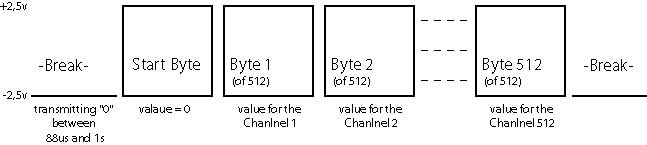
\includegraphics[width=0.9\textwidth,height=\textheight]{bilder/Clemens/dmx.jpg}
\caption{Darstellung des DMX-Signals\label{dmx-signal}}
\end{figure}

Der Vorteil dieses Protokolls ist, dass alle Empfänger nur an ein Kabel
angeschlossen werden müssen und die meist schon vorhandene
XLR-Verkabelung genutzt werden kann.\cite{dmx512/1990}

Ein Nachteil ist, dass bei vielen genutzten Kanälen das Signal und somit
auch die Refreshrate sehr gering wird. Das bedeutet, dass in der Praxis
DMX mit weniger Geräten betrieben werden sollte.\cite{dmx512/1990}

\hypertarget{anwendung-in-diesem-projekt}{%
\subsection{Anwendung in diesem
Projekt}\label{anwendung-in-diesem-projekt}}

In diesem Projekt wurde DMX als Schnittstelle zur Beleuchtung
integriert. Dadurch bleibt das System flexibel, so gibt der
Administrator bei der Installation nur an welcher Kanal, welchem
Scheinwerfer zuzuordnen ist. Weiters wird dadurch auch garantiert, dass
das System mit allen DMX-Stanadard konformen Scheinwerfern funktioniert.
Ein weiterer Vorteil, der sich durch die Integration des Protokolls
ergibt, ist, dass nicht nur Dimmer, sondern auch RGB- und
RGBW-Scheinwerfer gesteuert werden können. Die Art des Scheinwerfers
wird an der Anzahl der durch den Administrator angegebenen Kanäle pro
Scheinwerfer bestimmt. So ist es auch möglich, dass verschiedene Typen
gemischt werden können.

Wenn vom User der Befehl zur Änderung einer Einstellung an einem der
Scheinwerfer gesendet wird, wird im Hintergrund das zu diesem
Scheinwerfer passende Scheinwerfer-Objekt aufgerufen, welches über die
Php-Extension (siehe \ref{PHP-Extension}) und Ola (siehe \ref{Ola}) den
entsprechenden Wert des DMX-Kanals ändert.


\section{Infrarot}\label{Infrarot}

\renewcommand{\kapitelautor}{Autor: Clemens Scharwitzl}

\input{markdown/Clemens.md/Ir.md}

\section{Mischpult}\label{Mischpult}

\renewcommand{\kapitelautor}{Autor: Clemens Scharwitzl}

% \input{markdown/Clemens.md/myChapter.md}

\section{SQLite}\label{SQLite}

\renewcommand{\kapitelautor}{Autor: Clemens Scharwitzl}

% \input{markdown/Clemens.md/myChapter.md}

%%%%%%%%%%%%%%%%%%%%%% Chapter Frontend %%%%%%%%%%%%%%%%%%%%%
\chapter{Frontend}\label{Frontend}

\section{CSS}\label{CSS}

\renewcommand{\kapitelautor}{Autor: Dominik Nußbaumer}

    \hypertarget{flexbox}{%
\subsection{Flexbox}\label{flexbox}}

Flexbox, offiziell CSS Flexible Box Layout Module, ist eine neue Art und
ein neues Konzept um eindimensionale Layouts auf Webseiten umzusetzen.
Die herkömmliche Art Objekte auf einer Webseite zu positionieren ist,
fixe Positionen und Maße zu vergeben.

Doch bei Flexbox werden bestimmte Regeln festgelegt, diese machen das
Verhalten der Webseite vorhersagbar bei einer Veränderung der
Bildschirmgröße. Anschließend ist es dem Browser überlassen, die Breite,
Höhe, Position und Anordnung zu wählen.

\hypertarget{das-konzept}{%
\subsubsection{Das Konzept}\label{das-konzept}}

Die Grundidee ist es, dem Flex-Container die Möglichkeit zu geben, die
Maße der Elemente so zu verändern, dass der Platz auf unterschiedlichen
Bildschirmaufslösungen bestmöglich ausgenutzt ist. Um das zu erzielen
lässt das Elternelement die Kindelemente je nach Bedarf wachsen oder
schrumpfen.

\hypertarget{technische-spezifikation}{%
\subsubsection{technische
Spezifikation}\label{technische-spezifikation}}

Innerhalb eines \textless{}div\textgreater{} Tags können die einzelnen
Elemente ihre Größe ``flexibel'' verändern. Sie wachsen, um freien Platz
zu verwenden oder schrumpfen, um innerhalb des Elternobkjekts zu bleiben
und einen Overflow zu vermeiden. Der große Vorteil des Flexbox Layouts
ist die Richtungsunabhängigkeit. Dadurch ist es sehr flexibel, was
Orientierungsänderungen bei mobilen Geräten oder Auflösungsänderungen
auf Desktop Geräten betrifft.

\hypertarget{erkluxe4rung-anhand-eines-realen-beispiels}{%
\subsubsection{Erklärung anhand eines realen
Beispiels}\label{erkluxe4rung-anhand-eines-realen-beispiels}}

Auf dem Dashboard soll eine seitliche Navigation angezeigt werden, die
auf mobilen Geräten an den unteren Rand des Bildschirms wandert, siehe
Abbildung 1.

\begin{figure}
\centering
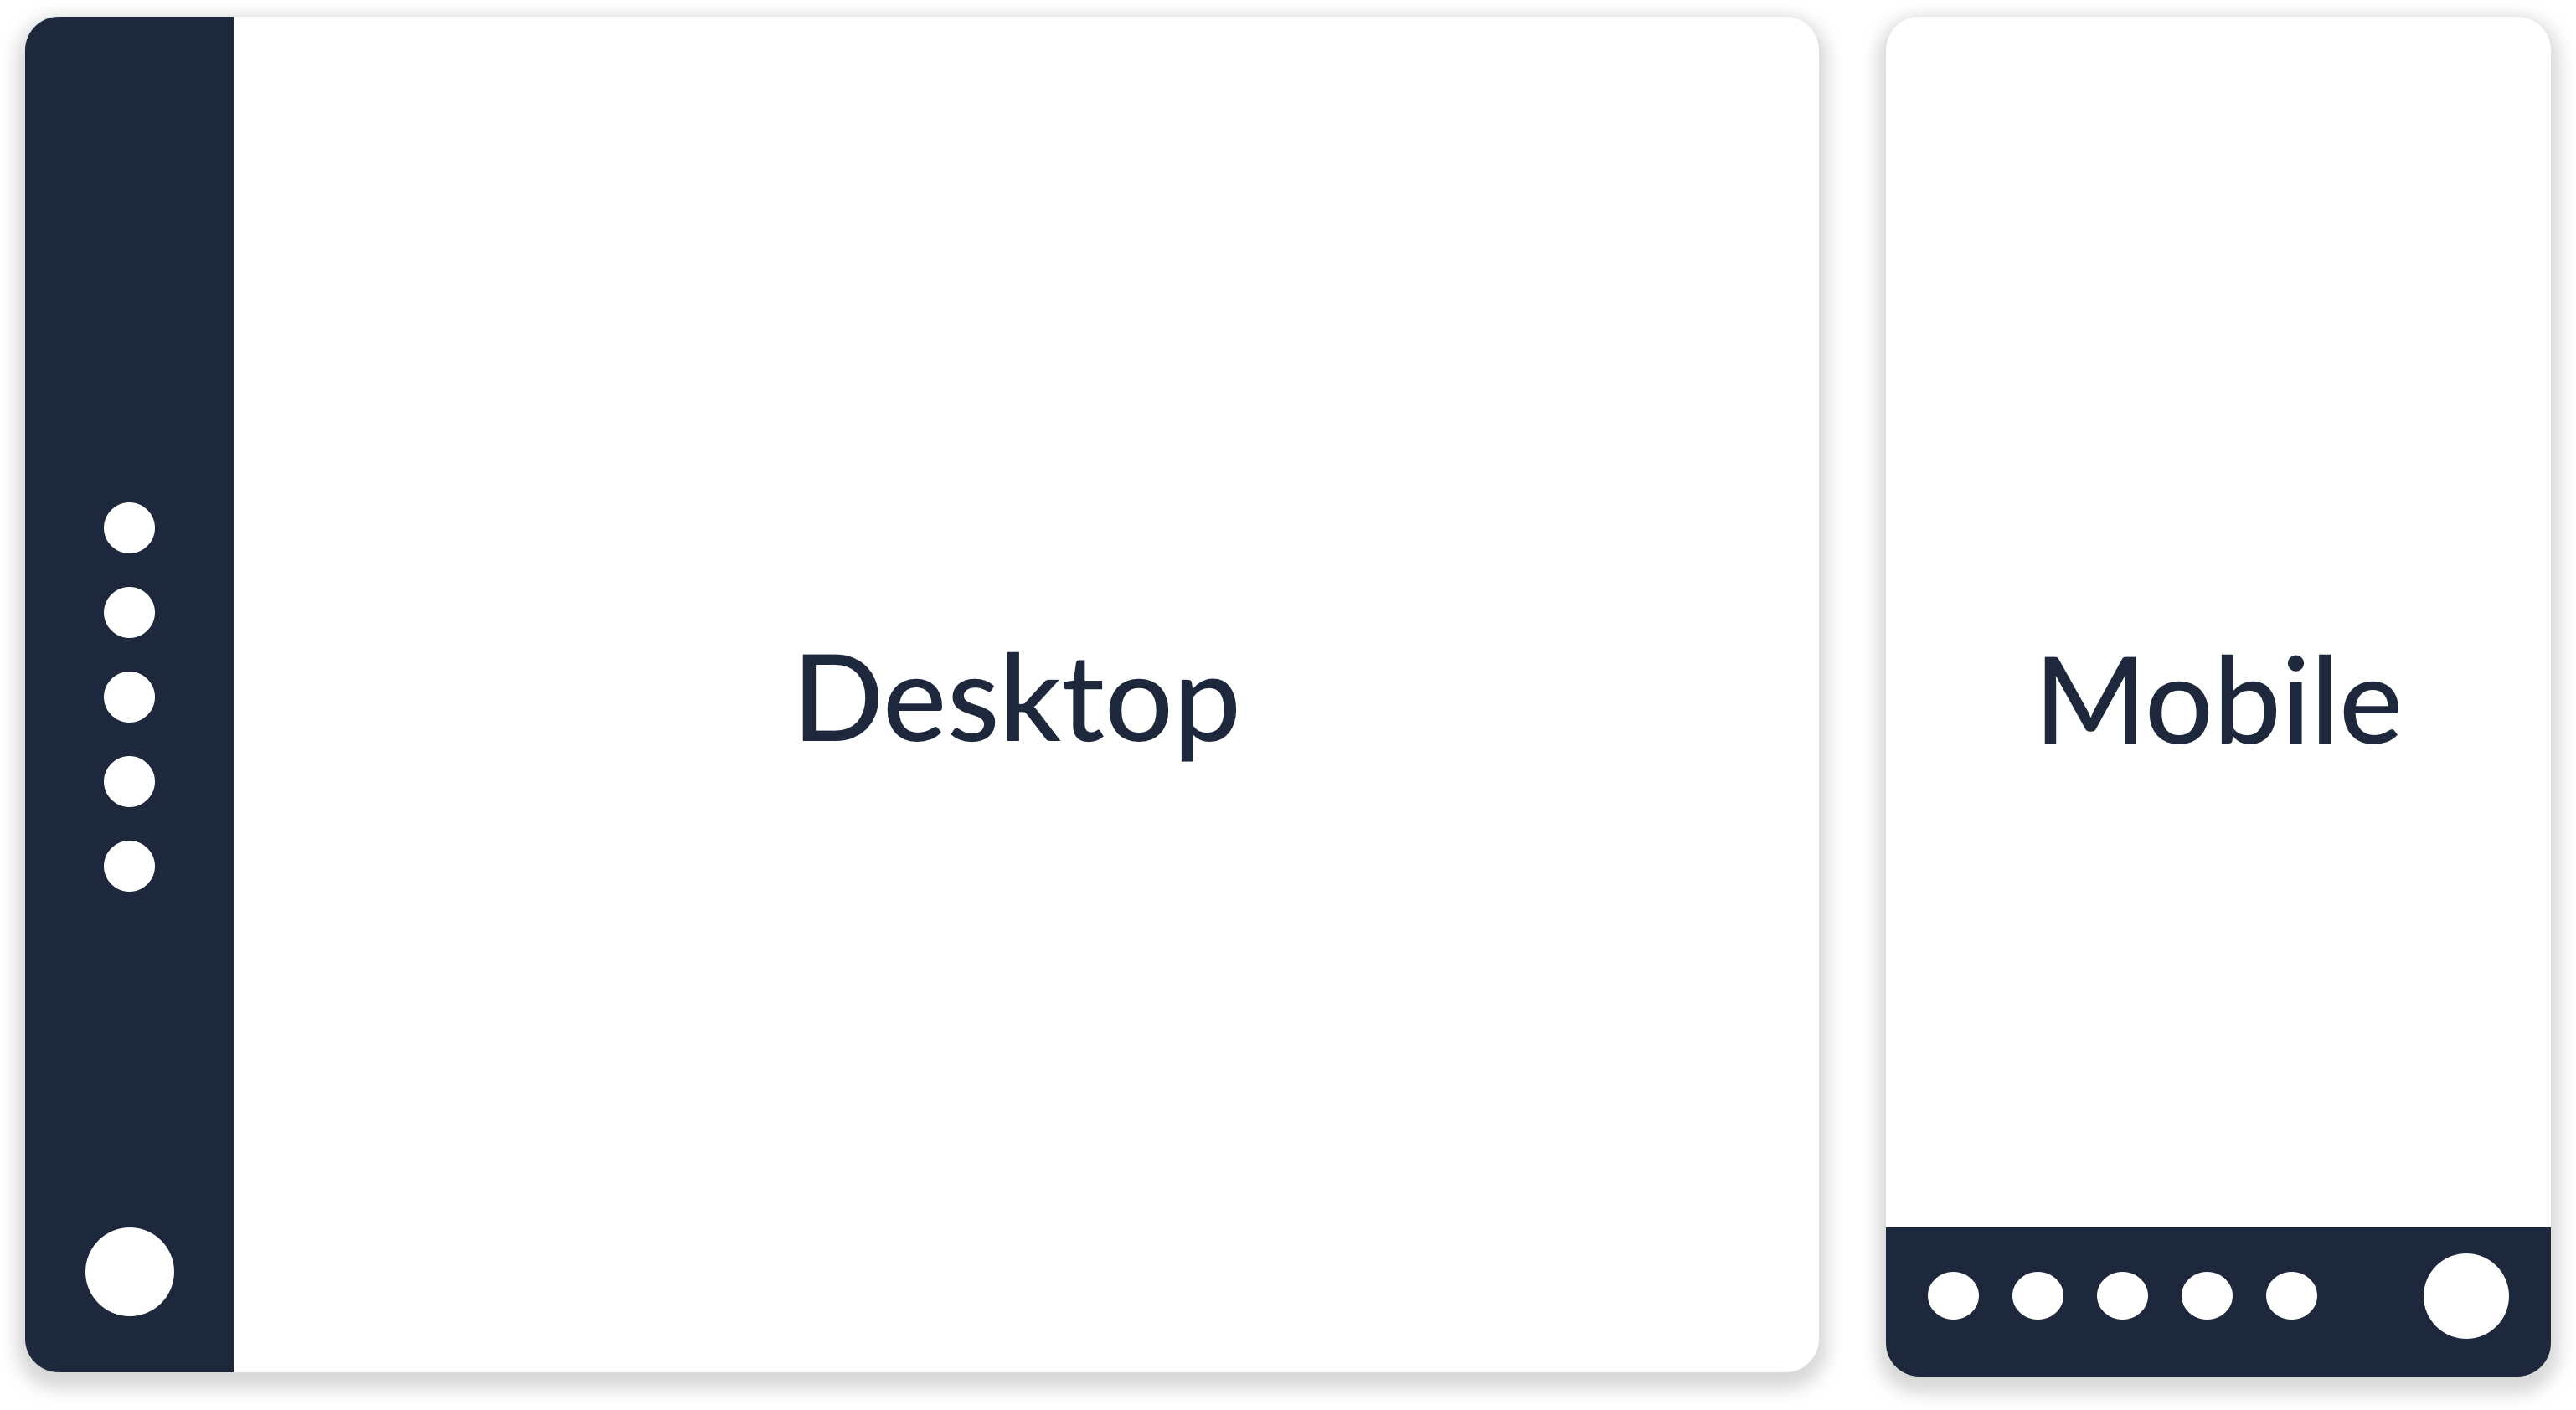
\includegraphics[width=0.9\textwidth,height=\textheight]{bilder/Dominik/Flexbox_Illustration_1.png}
\caption{Flexbox Beispiel}
\end{figure}

Mithilfe von Flexbox ist dieses Verhalten einfach zu erzielen. Ich
erstelle ein Elternelement mit folgenden Eigenschaften:

\begin{Shaded}
\begin{Highlighting}[]
\FunctionTok{.parent}\NormalTok{\{}
  \KeywordTok{display}\NormalTok{: flex;}
  \KeywordTok{overflow}\NormalTok{: }\DecValTok{hidden}\NormalTok{;}
\NormalTok{\}}
\end{Highlighting}
\end{Shaded}

Die Kindelemente dieser Flexbox werden auf der horizontalen Hauptachse
ausgerichtet. Der Overflow auf der X- und Y-Achse wird ausgeblendet. Die
Navigation auf der Seite ist in folgendem Code-Block beschrieben.

Dieses Element ist durch order:1 das erste Element in der Flexbox. Der
Overflow auf der Y-Achse ist versteckt, um die Leiste zu fixieren.
Weiters werden die Elemente innerhalb vertikal und horizontal zentriert
und sind entlang der Y-Achse positioniert.

\begin{Shaded}
\begin{Highlighting}[]
\FunctionTok{.side-nav}\NormalTok{\{}
  \KeywordTok{display}\NormalTok{: flex;}
  \KeywordTok{order}\NormalTok{: }\DecValTok{1}\NormalTok{;}
  \KeywordTok{justify-content}\NormalTok{: }\DecValTok{center}\NormalTok{;}
  \KeywordTok{align-items}\NormalTok{: }\DecValTok{center}\NormalTok{;}
  \KeywordTok{flex-direction}\NormalTok{: column;}
\NormalTok{\}}
\end{Highlighting}
\end{Shaded}

Das Inhaltselement hat order:2 damit es neben dem ersten auf der X-Achse
positioniert wird. Ebenso ist der Overflow auf der Y-Achse versteckt.

\begin{Shaded}
\begin{Highlighting}[]
\FunctionTok{.content}\NormalTok{\{}
  \KeywordTok{overflow-y}\NormalTok{: }\DecValTok{hidden}\NormalTok{;}
  \KeywordTok{display}\NormalTok{: flex;}
  \KeywordTok{justify-content}\NormalTok{: }\DecValTok{center}\NormalTok{;}
  \KeywordTok{flex-direction}\NormalTok{: column;}
  \KeywordTok{order}\NormalTok{: }\DecValTok{2}\NormalTok{;}
\NormalTok{\}}
\end{Highlighting}
\end{Shaded}

Damit die Navigation auf mobilen Geräten am unteren Rand positioniert
ist, benötigen wir eine Media Query. Mithilfe dieser können CSS-Stile
anhand von verschiedenen Eigenschaften wie z.B. Bildschirmauflösung oder
Seitenverhältnis manipuliert werden. Im untenstehenden Code-Block wird
dies veranschaulicht. Indem wir die Hauptachse des Flexbox
Elternelements auf die Y-Achse ändern, werden die beiden Kindelemente
nun vertikal verteilt. Damit nun auch die Navigation unter dem Inhalt
positioniert ist ändern wir die order auf 2. Weiters müssen die Höhe und
Breite angepasst werden.

\begin{Shaded}
\begin{Highlighting}[]
\ImportTok{@media}\NormalTok{ (}\KeywordTok{max-width}\NormalTok{: }\DecValTok{576px}\NormalTok{)\{}
  \FunctionTok{.parent}\NormalTok{\{}
    \KeywordTok{flex-direction}\NormalTok{: column; //changed}
\NormalTok{  \}}

  \FunctionTok{.side-nav}\NormalTok{\{}
      \KeywordTok{order}\NormalTok{: }\DecValTok{2}\NormalTok{;             //changed}
      \KeywordTok{width}\NormalTok{: }\DecValTok{100vw}\NormalTok{;         //changed}
      \KeywordTok{height}\NormalTok{: }\DecValTok{66px}\NormalTok{;         //changed}
\NormalTok{    \}}
\NormalTok{  \}}
\end{Highlighting}
\end{Shaded}

\hypertarget{muxf6glichkeiten}{%
\subsubsection{Möglichkeiten}\label{muxf6glichkeiten}}
{Autor: Dominik Nußbaumer}

    \hypertarget{css-grid}{%
\subsection{CSS Grid}\label{css-grid}}

CSS Grid, offiziell

\hypertarget{das-konzept}{%
\subsubsection{Das Konzept}\label{das-konzept}}

\hypertarget{technische-spezifikation}{%
\subsubsection{technische
Spezifikation}\label{technische-spezifikation}}

\hypertarget{erkluxe4rung-anhand-eines-realen-beispiels}{%
\subsubsection{Erklärung anhand eines realen
Beispiels}\label{erkluxe4rung-anhand-eines-realen-beispiels}}

\begin{Shaded}
\begin{Highlighting}[]
\FunctionTok{.parent}\NormalTok{\{}
  \KeywordTok{display}\NormalTok{: flex;}
  \KeywordTok{overflow}\NormalTok{: }\DecValTok{hidden}\NormalTok{;}
\NormalTok{\}}
\end{Highlighting}
\end{Shaded}

\hypertarget{muxf6glichkeiten}{%
\subsubsection{Möglichkeiten}\label{muxf6glichkeiten}}
{Autor: Dominik Nußbaumer}

    \input{markdown/Dominik.md/Grid_vs_Flexbox.md}{Autor: Dominik Nußbaumer}

\section{jQuery}\label{jQuery}

\renewcommand{\kapitelautor}{Autor: Dominik Nußbaumer}

% \input{markdown/Clemens.md/myChapter.md}

\section{Design}\label{Design}

\renewcommand{\kapitelautor}{Autor: Dominik Nußbaumer}

% \input{markdown/Clemens.md/myChapter.md}

%%%%%%%%%%%%%%%%%%%%%% Chapter Zusätzliches %%%%%%%%%%%%%%%%%%%%%
\chapter{Zusätzliches}\label{Zusätzliches}

\section{Bedienungsanleitung}\label{Bedienungsanleitung}

\renewcommand{\kapitelautor}{Autor: Clemens Scharwitzl}

% \input{markdown/Clemens.md/myChapter.md}

\section{Beleuchtungskonzept Konferenzsaal}\label{Beleuchtungskonzept-Konferenzsaal}

\renewcommand{\kapitelautor}{Autor: Clemens Scharwitzl}

% \input{markdown/Clemens.md/myChapter.md}

% \chapter{Ziele}

% Das erste Kapitel stellt die Ziele der DA (inkl. individuelle Ziele
% aller Mitarbeiter) da.\todo{viel Text schreiben}


% \chapter{Formatierung}

% wer hat diese Kapitel geschrieben oder leer
% \renewcommand{\kapitelautor}{Autor: Hans Huber}

% 
\section{Vorlagen}

In diesen Kapitel gibt es einige Muster für Dinge die oft vorkommen.
Und etwas Blindtext damit man auch volle Seiten sieht.


\subsection{Formatvorlagen}

Alle Formatierungen sollten mit Formatvorlagen vorgenommen werden.
Spätestens bei der Konvertierung in ein Ebook rächen sich diese \quotedblbase Sünden``:
Ebooks sind HTML Dokumente mit einer Formatierung mittels CSS.

Auch bei der Umwandlung in interaktive PDFs ist eine konsequente Formatierung
wichtig.


\subsection{Schriften und Absätze}

Hier findet man eine Beschreibung des Layouts -- Details folgen weiter
unten.
\begin{description}
\item [{Schrift:}] dieses \LaTeX{}-Dokument verwendet die Standardschriften.
Die Schriftgröße soll 12\,pt betragen.
\item [{Absatz:}] entweder verwendet man wie in \LaTeX{} einen etwas größeren
Seitenrand oder einen größeren Zeilenabstand. Beides sorgt für bessere
Lesbarkeit. Zwischen den Abätzen ist ein Abstand. Alternative: die
erste Zeile eines Absatzes wird etwas eingerückt (nicht die erste
Zeile nach einer Überschrift, nach einem Bild etc.) und bzw. oder
es gibt einen Abstand zwischen den Absätzen. Am Ende und Anfang einer
Seite sollten mindestens zwei Zeilen eines Absatzes sein (keine Schusterjungen\footnote{siehe \url{http://www.typolexikon.de/s/schusterjunge.html}}
und Hurenkinder\footnote{siehe \url{http://www.typolexikon.de/h/hurenkind.html}}).
\item [{Blocksatz:}] Alle Texte werden im Blocksatz gesetzt. Die Silbentrennung
ist dann obligatorisch.
\item [{Kapitelüberschriften:}] Überschriften erster Ordnung sollten auf
rechten Seiten beginnen. Über jeder Überschrift sollte ein Abstand
sein. Alle Überschriften müssen mit de nächsten Absatz \quotedblbase zusammengehalten``
werden -- keine einsamen Überschriften am Ende einer Seite.
\item [{Inhaltsverzeichnis:}] das Inhaltsverzeichnis sollte möglichst kompakt
sein. Als Gliederung dienen fette Hauptüberschriften und etwas Abstand
über den Zeilen.
\item [{Seitenformat:}] der Ausdruck erfolgt zweiseitig, ein entsprechender
Bundsteg ist zu berücksichtigen\footnote{Die Einstellung der Seitenränder ist keinesfalls beliebig. Sie sollte
bewährten Regeln folgen, {[}\ldots{}{]}. Die häufige Zielvorgabe
\quotedblbase Den Platz auf dem Papier möglichst gut ausnutzen``
ist keine typografische sondern eine extrem laienhafte Regel. aus
\citep{layout}}. Nach Rücksprache mit dem Betreuer kann auch eine einseitige Variante
gewählt werden. Bei Bedarf könne auch einzelne Seiten im Querformat
gesetzt werden.
\item [{Kopfzeile:}] die Kopfzeile sollte dieser Vorlage entsprechen. Falls,
nach Rücksprache mit dem Betreuer, der Ausdruck nur in Schwarz-weiß
erfolgt, kann das Logo entfallen.
\item [{Fußzeile:}] hier ist Platz für den Autor des Kapitels und die Seitennummer.
Wie bei technischen Publikationen üblich ist die Einleitung und die
Verzeichnisse mit römischen Seitennummern versehen. Das eigentliche
Dokument wird mit arabischen Ziffern nummeriert. Beide Nummerierungen
sind unabhängig voneinander und beginnen jeweils bei 1.
\item [{Autor:}] Jedes Kapitel muss auch einem Autor haben. Das sieht man
in der Fußzeile oder als Textbox in der Nähe der Überschrift. Alternativ
kann es im Anhang eine Liste geben. Das ist besonders wichtig wenn
es viele Beilagen, z.B. Handbücher ohne direkte Angabe des Autors,
gibt.
\item [{PDF:}] Die PDF Metainformation sollten richtig sein (Autor etc.)
-- siehe Datei/Eigenschaften. Links auf Webseiten, Verweise innerhalb
des Dokuments, das Inhaltsverzeichnis, die Fußnoten usw. sollten \quotedblbase klickbar``
sein.
\end{description}

\subsection{Bilder\label{sub:Bilder}}

Das Bild als Gleitobjekt ist genau hier, oder oben auf der Seite,
oder unten, aber immer zentriert mit Nummer und Beschreibung -- wenn
es sinnvoll ist auch mit Querverweis (siehe Abbildung \ref{Bild11}).
Durch Gleitobjekte, d.~h. Bilder oben oder unten auf der Seite statt
\quotedblbase genau hier``, werden halbleere Seiten durch besonders
große Bilder vermieden.

Wichtig: alle Bilder oder andere Medien z.~B. Screenshots, Audio
oder Video für EBooks und interaktive PDFs sollten mit einen entsprechenden
Quellennachweis versehen sein.

\begin{figure}[tbh]
\begin{centering}

\includegraphics[scale=0.6]{HTL3RLogoRGB}
\par\end{centering}

\caption{Ein Bild}
\label{Bild11}
\end{figure}



\subsection{Tabellen}

In der folgenden Tabelle sieht man: es gibt immer eine Nummer und
eine Beschreibung. Besonders längere Tabellen sollten eventuell als
Gleitobjekt am Ende oder Anfang einer Seite positioniert werden. Geht
die Tabelle über mehrere Seiten so ist die Überschrift zu wiederholen.

\begin{table}[h]
\begin{centering}
\begin{tabular}{|c|c|c|}
\hline 
Überschrift & Wert & noch einer\tabularnewline
\hline 
\hline 
1 & abc & Hallo\tabularnewline
\hline 
2 & def & Latex\tabularnewline
\hline 
\end{tabular}
\par\end{centering}

\caption{So eine tolle Tabelle}
\end{table}



\subsection{Formel}

Etwas Text als Überleitung zu einer Formel:

\selectlanguage{ngerman}%
\[
f(x)=\left\{ \begin{array}{cc}
\log_{8}x & x>0\\
0 & x=0\\
\sum_{i=1}^{5}\alpha_{i}+\sqrt{-\frac{1}{x}} & x<0
\end{array}\right.
\]


\selectlanguage{naustrian}%
Wenn man sehr viele Formeln hat sollte man diese auch nummerieren.
Besonders bei Verweisen ist das sehr sinnvoll.


\subsection{Sourcecode}

Sourcecode sollte in einer Schrift mit fixer Breite sein. Falls man
Verweise braucht sollte man die Listings auch nummerieren. 

% das kann auch ganz oben stehen
% das braucht man nur einmal
\lstset{numbers=left, numberstyle=\tiny, stepnumber=2, numbersep=5pt, showspaces=true, frame=single}
% einmal oder immer was anderes
\lstset{language=C}

% hier könnte man auch aus Dateien lesen
\begin{lstlisting} 
#include <stdio.h>

int main() 
{ 
  printf("Hello world\n"); 
} 
\end{lstlisting} 

Die genaue Formatierung ist freigestellt: Einstellungen wie bunt bzw.
fett, Markierung von Leerzeichen und Zeilennummerierung kann an den
Bedarf der Diplomarbeit angepasst werden. 

Beispiel Java mit anderen Einstellungen -- nur als Beispiel, in der
Diplomarbeit sollte man sich an eine einheitliches Format halten.
Bei längeren Listings muss man eventuell mit Umbrüchen rechnen, oder
man verwendet einen Rahmen der frei angeordnet werden kann (\siehe{sub:Bilder}).

% Einstellungen für die fogenden Listings
% entweder mit \begin{listing} oder in Lyx als Programmlisting
\lstset{numbers=right, numberstyle=\tiny, stepnumber=2, numbersep=5pt, showspaces=false, frame=single}
\lstset{language=Java}

Achtung \LaTeX{}-User: Listing kann keine Umlaute, aber unter \citep{listingtipp}
gibt es eine Lösung.

\begin{lstlisting}[caption={Java Beispiel},captionpos=b]
import java.awt.*;  
import java.awt.event.*;
public class AL extends Frame
                 implements WindowListener, ActionListener {
  TextField text = new TextField(20);
  Button b;    
  private int numClicks = 0;
 
  public static void main(String[] args) {
    AL myWindow = new AL("My first window");
    myWindow.setSize(350,100);
    myWindow.setVisible(true);    
  } 
}
\end{lstlisting}

Hinweis: Pandoc erzeugt automatisch bunte Listings.

\subsection{Fachbegriffe}

Fachbegriffe in einer Fremdsprache oder Kommandos sollten einheitlich
gekennzeichnet werden. Bei Latex verwendet man dazu \quotedblbase logisches
Markup``, bei Word oder Open/Libre-office wird all diesen Wörtern
wird eine Vorlage zugewiesen, das Aussehen wird dann an einer Stelle
zentral festgelegt. 

Als Beispiel soll \emph{Text to Speech}\index{Text to Speech: Umwandlung von Texten in Sprache}
dienen. Solche Wörter sollte natürlich in ein Glossar aufgenommen
werden. 

Oder der Befehl \strong{dir} für die Kommandozeile. Die Angabe von
Dateinamen sollte auch einheitlich sein: entweder \emph{/etc/passwd}
oder \strong{C:\textbackslash{}system32}.


\subsection{Zitieren}

Die Quellenangabe kann in Form eines Vollbelegs in der Fußnote\footnote{aus Zitat --- Wikipedia, Die freie Enzyklopädie, \url{http://de.wikipedia.org/w/index.php?title=Zitat},
Abgerufen 2014-09-14}(bei technischen Dokumenten eher unüblich) oder als Kurzbeleg am Schluss
der gesamten Arbeit aufgeführt werden. Beim Kurzbeleg sind dabei verschiedene
Formen üblich. Der platzsparendste, aber am wenigsten aussagekräftige
Zitierstil ist die fortlaufende Nummerierung aller zitierten Quellen
{[}123{]} -- diese wird auch in dieser Vorlage verwendet.

Alternativen -- nur in begründeten Ausnahmefällen: Insbesondere in
der Informatik üblich ist eine Kombination der ersten drei Buchstaben
des Autorennamens und der letzten beiden Ziffern des Erscheinungsjahres
(z. B. „The04“ für Theisen 2004). Wohl am weitesten verbreitet ist
der vollständige Verfassernamen mit Erscheinungsjahr, wobei mehrere
Quellen desselben Autors innerhalb eines Jahres durch fortlaufende
Buchstaben kenntlich gemacht werden (z. B. „Theisen 2004c“). Weniger
üblich, aber am aussagekräftigsten ist die Quellenangabe unter Hinzufügung
eines Schlagwortes, das den mit der Materie vertrauten Leser zumeist
bereits die zitierte Quelle erkennen lässt, z. B. in der Form „Theisen
(Wissenschaftliches Arbeiten, 2004)“.

Obwohl mehrere Zitierstile bzw. Zitiertechniken zur Verfügung stehen,
werden in einem Dokument üblicherweise nicht mehrere verwendet; ein
ausgewählter Zitierstil wird im gesamten Dokument konsequent beibehalten.
Ein gute Übersicht bietet \citep{wiki:zitat}.

Auch unter \url{http://www.diplomarbeiten-bbs.at/zitation-plagiate}
gibt es gute Informationen zum Thema.


\subsubsection{Quellenverzeichnis}

Unter \LaTeX{} kann das Programm Bib\TeX{} zur Erstellung von Literaturangaben
verwendet werden. 
\begin{itemize}
\item Links auf Wikipedia sollten vermieden werden.
\item Jeder Link sollte mit einem Abfragedatum versehen sein.
\item Das Literaturverzeichnis kommt an das Ende des Dokuments.
\end{itemize}
Viele Details dazu findet man bei \citep{wiki:zitat}.


\subsubsection{Rechtliches zum Zitieren}

Achtung: nicht gekennzeichnete Zitate (Plagiate) führen zu einer negativen
Beurteilung der Diplomarbeit.

Nach \citep{wiki:quelle}:

§ 57 des österreichischen Urheberrechtsgesetzes\citep{ris57} enthält
detaillierte Vorschriften über die Quellenangabe, unter anderem: Werden
Stellen oder Teile von Sprachwerken nach §\,46 vervielfältigt, so
sind sie in der Quellenangabe so genau zu bezeichnen, dass sie in
dem benutzten Werke leicht aufgefunden werden können. In den Erläuterungen
(ErlRV) heißt es: Bei Entlehnungen aus umfangreichen Werken muss also
in der Quellenangabe auch die Seite, der Abschnitt, das Kapitel oder
der Akt, wo sich die entlehnte Stelle befindet, angeführt werden (Dillenz,
Materialien zum österreichischen Urheberrecht, 134, zitiert nach \citep{dittrich},
S. 621)

2002 nahm der österreichische OGH zur Frage der Quellenangabe in der
Entscheidung Riven Rock Stellung: Nach § 57 Abs 4 UrhG bedarf die
Unterlassung einer Quellenangabe der Rechtfertigung durch die im redlichen
Verkehr geltenden Gewohnheiten und Gebräuche. Bei Auslegung dieser
Bestimmung ist eine Abwägung der Interessen des Urhebers mit jenen
des zur freien Werknutzung Berechtigten nach dem Verständnis loyaler,
den Belangen des Urhebers mit Verständnis gegenübertretenden, billig
und gerecht denkenden Benutzern (Vinck aaO § 63 Rz 2) geboten und
danach zu beurteilen, ob dem freien Werknutzer neben der Nennung des
Autors/Verlags auch die Nennung des Namens des Übersetzers von in
einer Rundfunksendung verlesenen Roman-Zitaten zumutbar ist.


\section{Inhalt}


\subsection{Aussagen}

Alles im Buch sollte man in folgende drei Typen einteilen:
\begin{enumerate}
\item Stand der Technik -- Quelle notwendig
\item selbst gemacht -- Verweis wie und wo
\item Meinung -- als eigene Meinung bzw. Einschätzung kennzeichnen
\end{enumerate}

\subsection{Bad Practice}

Was man vermeiden sollte -- diese Dinge führen zur Mehrarbeit und
verursachen zusätzlichen Stress in der hektischen Zeit knapp vor dem
Abgabetermin.


\paragraph{Stil}
\begin{itemize}
\item Extrem lange, geschachtelte Sätze und/oder endlose Textpassagen ohne
Gliederung durch Absätze.\nopagebreak

\begin{itemize}
\item Vielleicht bzw. sinnvollerweise lassen Sie den Text auch von einer
\quotedblbase außenstehenden Person`` lesen. 
\end{itemize}
\item Aufzählungen im Text statt Listen. Wie man hier sieht dürfen bei Listen
auch mehrere Sätze stehen.
\item \uline{Unterstreichen} ist ein Relikt aus \quotedblbase Schreibmaschinen-Zeiten``.
\item Eine Diplomarbeit ist keine Erzählung. Natürlich kann man als \quotedblbase ich``
oder \quotedblbase wir`` auf \quotedblbase unsere Probleme`` eingehen,
aber im Allgemeinen ist ein formaler, beschreibender und technischer
Stil einzuhalten.
\item Eine Diplomarbeit ist auch keine Email oder SMS: Schreiben Sie ganze
Sätze ohne kryptische Abkürzungen und Smileys.
\item Ein Mindestmaß an Interpunktion wird vorausgesetzt. Eventuell lassen
Sie den Text durch eine kundige Person Ihres Vertrauens korrigieren.
\item Es gibt viele verschiedene Striche, und alle sehen verschieden aus:
Gedankenstriche, Bindestriche und Minus kommen in einer Diplomarbeit
häufig vor.
\item Weitere Wörter die Ihren Betreuer verzweifeln lassen -- natürlich
nur bei übermäßiger Verwendung

\begin{itemize}
\item Welcher/Welches, Hierbei
\end{itemize}
\end{itemize}

\paragraph{Technik}
\begin{itemize}
\item (viele) händische Formatierungen statt Formatvorlagen.
\item zusätzliche manuelle Seitenumbrüche oder Leerzeilen für ein \quotedblbase schöneres``
Layout. Es gibt bei den Absatzformatierungen tolle Möglichkeiten für
Abstände vor und nach einem Absatz bzw. zum Beeinflussen des Textflusses.
Mittels \zB \code{\textbackslash{}needspace\{2cm\}} kann man für
\textit{genügend} Platz sorgen.
\item Arbeiten Sie mit dem Programm statt gegen das Programm:

\begin{itemize}
\item Verweise als fixer Text. Nutzen Sie die Möglichkeiten der Textverarbeitung.
\item Dinge die \quotedblbase kompliziert`` einzugeben sind, sind meist
falsch -- richtige Lösungen sind in allen Programmen auch \quotedblbase leicht``
zu erreichen\footnote{Oder Sie verwenden ein für Ihre Zwecke schlecht geeignetes Programm.}.
\end{itemize}
\item Kontrollieren Sie beim fertigen PDF die Angaben unter Datei / Eigenschaften
-- dort sollten sinnvolle Dinge stehen. Bei Latex wird dazu das Paket
\texttt{\code{\texttt{hyperref}}} verwendet.
\end{itemize}

\section{Details zu Formatierung}


\subsection{Schriftarten}

Die Word- und Libreoffice-vorlage verwenden etwas andere Schriften
als das Latex Dokument.


\section{Beispiele}


\subsection{Zitieren mit Latex}

Am Beispiel der URL \url{http://de.wikibooks.org/wiki/LaTeX-Kompendium}
und des Buches \quotedblbase \LaTeX{}: Einführung``.

Man braucht eine \texttt{.bib} Datei mit den notwendigen Informationen:

\begin{lstlisting}[language={[LaTeX]TeX}]
@book{kopka1991latex,
  title={LaTeX: Einfuehrung},
  author={Kopka, Helmut and Rahtz, Sebastian},
  volume={2},
  year={1991},
  publisher={Addison-Wesley} 
}

@online{latexKomp,
  author = {},
  title ={LaTeX-Kompendium - Wikibooks, Sammlung freier Lehr-, 
Sach- und Fachbuecher},
  url = {http://de.wikibooks.org/wiki/LaTeX-Kompendium},
  lastchecked = {2014.09.14},
}
\end{lstlisting}


Diese Einträge werden dann im Text verwendet: \texttt{\textbackslash{}cite\{kopka1991latex\}
}und das Ergebnis sieht dann so \citep{kopka1991latex} und so \citep{latexKomp}
aus. Gleichzeitig erscheinen diese Einträge auch im Literaturverzeichnis
am Ende des Dokuments.


\subsection{Formatierungen }

Der Autor kann natürlich auch eingreifen und zum Beispiel\\
Zeilenumbrüche erzwingen und \\
\\
Leerzeilen -- aber das sollte man nicht machen. \newpage{}

Ein Seitenumbruch kostet mich auch nicht mehr als einen müden Lacher,
ist aber noch seltener wirklich sinnvoll.

Schriftgrößen:
\begin{itemize}
\item {\tiny{}tiny} 
\item {\scriptsize{}scriptsize} 
\item {\footnotesize{}footnotesize} 
\item {\small{}small} 
\item normalsize 
\item {\large{}large} 
\item {\Large{}Large} 
\item {\LARGE{}LARGE} 
\item {\huge{}huge} 
\item {\Huge{}Huge} \end{itemize}
\begin{enumerate}
\item Nummerierungen
\item sind 
\item auch 
\item easy
\end{enumerate}
\textbf{bissl was fettes} \textit{italienisches} \uline{für unten
drunter}.




% \chapter{Planung}

% Das komplette nächste Kapitel wird in der externen Datei diplomarbeit2.tex gespeichert.
% Es wird an dieser Stelle im Dokument eingebaut.
% Damit ist es möglich, mehrere Personen an diverse Teile der Diplomarbeit arbeiten zu lassen.

% \hypertarget{kapitel-aus-der-anderen-datei}{%
\section{Kapitel aus der anderen
Datei}\label{kapitel-aus-der-anderen-datei}}

Dieses Kapitel wurde als \emph{diplomarbeit2.md} geschrieben und dann
mit \emph{pandoc} in \TeX~umgewandelt.

\begin{Shaded}
\begin{Highlighting}[]
\ExtensionTok{pandoc}\NormalTok{ --listings -s diplomarbeit2.md -o diplomarbeit2.tex }
\end{Highlighting}
\end{Shaded}

Wie man sieht ist das ganz einfach, sogar Listings sind möglich. Weitere
Optionen sind möglich bzw. sinnvoll -- siehe Kapitel \ref{skripts},
Seite \pageref{skripts}. Man beachte die von Pandoc automatisch
genmerierten Label für Querverweise.

Vorschlag zur Durchführung:

\begin{itemize}
\tightlist
\item
  ein Ordner mit den Pandoc-Dateien
\item
  ein Skript/Batch-Datei erzeugt daraus die Latex-Dateien

  \begin{itemize}
  \tightlist
  \item
    in einem neuen Ordner -- das erhöht die Übersichtlichkeit
  \end{itemize}
\item
  die Latex-Dateien werden dann in das Hauptdokument eingebunden
\end{itemize}

Und nun zu einem Bild.

\begin{figure}
\centering

\includegraphics{HTL3RLogo.png}
\caption{Der Text steht unterhalb}
\end{figure}

Man kann auch die Breite aber auch angeben.

\begin{figure}
\centering

\includegraphics[width=12cm]{HTL3RLogo.png}
\caption{Das kleinere Bild}
\end{figure}

Oder ganz klein

\begin{figure}
\centering

\includegraphics[width=2cm]{HTL3RLogo.png}
\caption{Das ganz kleine Bild}
\end{figure}

Auch Listen sind kein Problem, wichtig sind nur Leerzeilen zwischen den
Listenpunkten. Hier sieht man eine einfache Aufzählung.

\begin{itemize}
\item
  wichtig
\item
  auch ganz lange Texte können bei Listen geschrieben werden.

  Sogar mehrere Absätze sind möglich.
\item
  Ende der Liste.
\end{itemize}

Welches Zeichen am Anfang der Liste steht ist dabei leicht einzustellen,
im \emph{pandoc} Manual gibt es nähere Infos:

\begin{enumerate}
\def\labelenumi{\arabic{enumi}.}
\item
  eins
\item
  zwei

  \begin{enumerate}
  \def\labelenumii{\roman{enumii}.}
  \tightlist
  \item
    zwei eins -- Mindestens 4 Zeichen eingerückt
  \item
    zwei zwei
  \end{enumerate}
\item
  drei. \emph{Pandoc} zählt richtig, das Zeichen am Anfang der Zeile ist
  nur ein Muster!
\end{enumerate}

Mit den richtigen Optionen werden URLs automatisch richtig dargestellt
und sind im fertigen Pdf auch \emph{klickbar}:
\url{http://pandoc.org/README.html}


% \hypertarget{was-man-einstellen-kann}{%
\section{Was man einstellen kann}\label{was-man-einstellen-kann}}

Einige \emph{Dinge} kann man bei der Diplomarbeit auch noch anpassen.
Einiges ist sogar in der lyx- bzw. tex-Datei schon vorgesehen -- bitte
den Anfang des Source-Codes aufmerksam lesen.

\hypertarget{inhaltkapitel}{%
\subsection{Inhalt/Kapitel}\label{inhaltkapitel}}

Einige Ideen zur Gliederung der Arbeit gibt es unter
\url{http://www.diplomarbeiten-bbs.at/} \footnote{\url{http://www.diplomarbeiten-bbs.at/erstellung/durchf\%C3\%BChrung/gliederung-der-diplomarbeit-und-formale-vorgaben-0}}

\hypertarget{einseitigzweiseitig}{%
\subsection{Einseitig/zweiseitig}\label{einseitigzweiseitig}}

Korrekturexemplar immer einseitig drucken. Das fertige Buch ist dann
beidseitig zu drucken.

Begründete Abweichungen sind bitte mit dem Betreuer abklären -- die
Vorlage ist dann anzupassen (Überschriften, Vorlage für Kaitel, Bundsteg
usw.).

\hypertarget{farben}{%
\subsection{Farben}\label{farben}}

\begin{itemize}
\tightlist
\item
  Deckblatt mit Logo immer in Farbe
\item
  Farbausdrucke sind viel teurer -- Notwendigkeit prüfen und mit dem
  Betreuer abklären.
\item
  am aufwändigsten: ein paar Seiten in Farbe
\item
  falls Schwarz-Weiß: kein Logo beim laufenden Text
\end{itemize}

\hypertarget{autor}{%
\subsection{Autor}\label{autor}}

Bei der Diplomarbeit muss jeder Text einem Autor zuzuordnen sein. Man
kann das wie in der Vorlage in der Fußzeile machen. Alternativ kann man
auch eine Übersicht als Anhang eingefügt werden -- bitte mit dem
Betreuer abklären.

\hypertarget{absuxe4tze}{%
\subsection{Absätze}\label{absuxe4tze}}

\hypertarget{einzug}{%
\subsubsection{Einzug}\label{einzug}}

Den Beginn eines neuen Absatzes kann man durch Abstand oder durch
Einrücken kennzeichnen.

Diese Einstellung wird in der Vorlage bzw. im Header gemacht:

\begin{Shaded}
\begin{Highlighting}[]
\CommentTok{%\textbackslash{}parindent0pt % auskommentieren, wenn keine Einrueckung der }
               \CommentTok{% ersten Absatzzeile gewuenscht}
\CommentTok{%\textbackslash{}parskip1.5ex plus0.5ex minus0.5ex % flexibler Absatzabstand}
\end{Highlighting}
\end{Shaded}

Die Option \texttt{parskip=half} bei \texttt{documentclass} ersetzt
bereits den Absatzeinzug durch einen Absatzabstand.

oder \url{http://ctan.org/pkg/parskip}

\begin{Shaded}
\begin{Highlighting}[]
\BuiltInTok{\textbackslash{}usepackage}\NormalTok{[parfill]\{}\ExtensionTok{parskip}\NormalTok{\}}
\end{Highlighting}
\end{Shaded}

\hypertarget{noch-schuxf6ner}{%
\subsubsection{noch schöner}\label{noch-schuxf6ner}}

\url{http://www.khirevich.com/latex/microtype/}

\hypertarget{aufzuxe4hlungen}{%
\subsection{Aufzählungen}\label{aufzuxe4hlungen}}

Man kann die Einrückung und vieles mehr anpassen:

\begin{Shaded}
\begin{Highlighting}[]
\BuiltInTok{\textbackslash{}usepackage}\NormalTok{\{}\ExtensionTok{enumitem}\NormalTok{\}}
\FunctionTok{\textbackslash{}setlist}\NormalTok{[1]\{labelindent=}\FunctionTok{\textbackslash{}parindent}\NormalTok{\}}
\FunctionTok{\textbackslash{}setlist}\NormalTok{\{align=left\}}
\FunctionTok{\textbackslash{}setlist}\NormalTok{[itemize]\{leftmargin=*\}}

\CommentTok{% oder: }
\FunctionTok{\textbackslash{}setlength\textbackslash{}partopsep}\NormalTok{\{0.5ex\}}
\end{Highlighting}
\end{Shaded}

\hypertarget{warnungen}{%
\subsection{Warnungen}\label{warnungen}}

\begin{Shaded}
\begin{Highlighting}[]
\FunctionTok{\textbackslash{}sloppy}  \CommentTok{% etwas laxere Abstandskontrolle (weniger Fehlermeldungen)}
\end{Highlighting}
\end{Shaded}

\hypertarget{listings}{%
\subsection{Listings}\label{listings}}

Sonderzeichen:

\url{http://en.wikibooks.org/wiki/LaTeX/Source_Code_Listings\#Encoding_issue}

Anpassen:

\url{http://stackoverflow.com/questions/1965702/how-to-mark-line-breaking-of-long-lines}

\url{http://www.bollchen.de/blog/2011/04/good-looking-line-breaks-with-the-listings-package/}

\hypertarget{zitierstil}{%
\subsection{Zitierstil:}\label{zitierstil}}

Bitte mit dem Betreuer abklären.

\begin{itemize}
\tightlist
\item
  plaindin - mit nummern {[}1{]}
\item
  alphadin - mit Text+Jahr {[}Hor99{]}
\end{itemize}

\hypertarget{glossar}{%
\subsection{Glossar}\label{glossar}}

\begin{itemize}
\tightlist
\item
  \url{http://texwelt.de/wissen/fragen/10496/glossaries-alle-symbole-nur-verwendete-abkurzungen-anzeigen}
\item
  \url{http://en.wikibooks.org/wiki/LaTeX/Glossary} für die
  verschiedenen Formen
\end{itemize}

\hypertarget{ausdruck-zu-weit-obenunten}{%
\subsection{Ausdruck zu weit
oben/unten}\label{ausdruck-zu-weit-obenunten}}

Man kann das Layout anpassen: Position auf Seite

\begin{Shaded}
\begin{Highlighting}[]
\FunctionTok{\textbackslash{}voffset}\NormalTok{10mm}
\end{Highlighting}
\end{Shaded}

\hypertarget{urls}{%
\subsection{URLs}\label{urls}}

Man kann/sollte das \texttt{hyperref}-Paket anpassen, die bunten Links
kann man ausschalten.

\begin{Shaded}
\begin{Highlighting}[]
\FunctionTok{\textbackslash{}hypersetup}\NormalTok{\{breaklinks=true,}
\NormalTok{bookmarks=true,}
\NormalTok{pdfauthor=\{Mein Name\},}\CommentTok{% <------------------- anpassen!}
\NormalTok{pdftitle=\{Die Diplomarbeit\},}\CommentTok{% <------------------- anpassen!}
\NormalTok{colorlinks=true,}
\NormalTok{citecolor=blue,}
\NormalTok{urlcolor=blue,}
\NormalTok{linkcolor=magenta,}
\NormalTok{pdfborder=\{0 0 0\}\}}

\FunctionTok{\textbackslash{}urlstyle}\NormalTok{\{same\}}
\end{Highlighting}
\end{Shaded}

\hypertarget{pandoc-caption-mit-verweis}{%
\subsection{Pandoc-Caption mit
Verweis}\label{pandoc-caption-mit-verweis}}

siehe \url{https://github.com/chiakaivalya/thesis-markdown-pandoc}

This is how you insert figures using markdown. Also how to insert
citations copied over from your bibliography manager (I specifically
used Pandoc Citations in Papers).

\begin{verbatim}
![Figure from Walczak, 2010[@Walczak:2010uk]. 
    \label{mitosis} ](figures/mitosis_Walczak.pdf)
\end{verbatim}

\hypertarget{seitennummern}{%
\subsection{Seitennummern}\label{seitennummern}}

\url{http://www.golatex.de/wiki/\%5Cfrontmatter}

\begin{Shaded}
\begin{Highlighting}[]
\FunctionTok{\textbackslash{}frontmatter} \CommentTok{% switches to roman numbering}
\FunctionTok{\textbackslash{}mainmatter}
\FunctionTok{\textbackslash{}backmatter}
\end{Highlighting}
\end{Shaded}

\hypertarget{vorlagen}{%
\subsection{Vorlagen}\label{vorlagen}}

\hypertarget{tu-wien-informatik}{%
\subsubsection{TU Wien -- Informatik}\label{tu-wien-informatik}}

\begin{itemize}
\tightlist
\item
  \url{https://gitlab.cg.tuwien.ac.at/auzinger/vutinfth.git}

  \begin{itemize}
  \tightlist
  \item
    super Vorlage und Build-Skripts (auch für Windows)
  \end{itemize}
\item
  \url{http://www.informatik.tuwien.ac.at/dekanat/abschluss-master}
\item
  \url{http://www.informatik.tuwien.ac.at/fakultaet/informatik-code-of-ethics.pdf}
\item
  Alte Vorlage

  \begin{itemize}
  \tightlist
  \item
    \url{http://ieg.ifs.tuwien.ac.at/~aigner/download/tuwien.sty}
  \item
    von dort sind die Abkürzungen kopiert
  \end{itemize}
\end{itemize}

\hypertarget{andere}{%
\subsubsection{Andere}\label{andere}}

\begin{itemize}
\tightlist
\item
  \url{https://www.ctan.org/tex-archive/macros/latex/contrib/etdipa?lang=de}
\item
  \url{https://github.com/Digital-Media/HagenbergThesis}

  \begin{itemize}
  \tightlist
  \item
    enthält viele Tipps
  \end{itemize}
\item
  \url{https://github.com/philipmichel/vorlage-diplomarbeit-latex/blob/master/diplom.pdf}
\end{itemize}

\hypertarget{tipps-zur-diplomarbeit}{%
\section{Tipps zur Diplomarbeit}\label{tipps-zur-diplomarbeit}}

\hypertarget{source}{%
\subsection{Source}\label{source}}

\begin{itemize}
\tightlist
\item
  mit Java/Python/*-doc
\item
  sinnvolle Namen
\item
  Codierrichtlinien eingehalten

  \begin{itemize}
  \tightlist
  \item
    definiert?
  \item
    welche?
  \end{itemize}
\end{itemize}

\hypertarget{buch}{%
\subsection{Buch}\label{buch}}

\begin{itemize}
\item
  einheitliche Formatierung

  \begin{itemize}
  \tightlist
  \item
    Formatvorlage eingehalten
  \end{itemize}
\item
  Layout

  \begin{itemize}
  \tightlist
  \item
    kein halb-leeren Seiten
  \item
    wichtig bei Bildern und Listings
  \end{itemize}
\item
  Grammatik + Rechtschreibung
\item
  Irgendwie sollte man ein (einheitliches) Bild vom Leser haben:\newline
  Negaivbeispiel:

  \begin{itemize}
  \tightlist
  \item
    einerseits eine Dummy dem man \texttt{mdir} erklären muss
  \item
    andererseits kann er Python-Pakete installieren
  \end{itemize}
\end{itemize}

\hypertarget{umfang}{%
\subsubsection{Umfang}\label{umfang}}

\begin{itemize}
\tightlist
\item
  ohne Bilder aus dem Web bzw. Füllbilder
\end{itemize}

\hypertarget{formulierungen}{%
\subsection{Formulierungen}\label{formulierungen}}

NICHT:

\begin{itemize}
\tightlist
\item
  romanartige Erzählungen
\item
  seitenlange Installationsanweisungen statt Link auf Anleitung im Web
\end{itemize}

\hypertarget{listings-1}{%
\subsection{Listings}\label{listings-1}}

\begin{itemize}
\item
  wenig
\item
  ohne Kommentare

  \begin{itemize}
  \tightlist
  \item
    dafür mit Erklärung
  \item
    mit Verweis auf File
  \end{itemize}
\item
  UML Diagramme als Ergänzung
\item
  Anordung: Floating
\end{itemize}

\hypertarget{bilder}{%
\subsection{Bilder}\label{bilder}}

\begin{itemize}
\tightlist
\item
  Floating
\item
  Quellenangabe
\end{itemize}

\hypertarget{versionsverwaltung}{%
\subsection{Versionsverwaltung}\label{versionsverwaltung}}

\begin{itemize}
\tightlist
\item
  je unabhängigen Teilprojekt
\item
  sinnvolle Kommits (Nachrichten)
\item
  regelmäßig
\end{itemize}

\hypertarget{ppm}{%
\subsection{PPM}\label{ppm}}

\begin{itemize}
\tightlist
\item
  Entscheidung: Wieviel?
\item
  NICHT unreflektierte Analysen vom Projektstart im Anhang
\end{itemize}

\hypertarget{quellen}{%
\subsection{Quellen}\label{quellen}}

\begin{itemize}
\tightlist
\item
  alle Tools inkl. Versionsnummer
\item
  alle Zitate bzw. übernommenen Meinungen
\item
  Datenblätter \ua
\end{itemize}

\hypertarget{skripts}{%
\section{Skripts}\label{skripts}}

\hypertarget{pandoc-nach-latex}{%
\subsection{Pandoc nach Latex}\label{pandoc-nach-latex}}

\begin{Shaded}
\begin{Highlighting}[]
\CommentTok{#! /bin/bash}
\CommentTok{#set -x}
\CommentTok{#set -v}
\KeywordTok{set} \ExtensionTok{-e}

\VariableTok{PANDOCMODULES=}\NormalTok{markdown+auto_identifiers}
\VariableTok{PANDOCMODULES=$\{PANDOCMODULES\}}\NormalTok{+definition_lists}
\CommentTok{#PANDOCMODULES=$\{PANDOCMODULES\}+compact_definition_lists}
\VariableTok{PANDOCMODULES=$\{PANDOCMODULES\}}\NormalTok{+fenced_code_attributes}
\VariableTok{PANDOCMODULES=$\{PANDOCMODULES\}}\NormalTok{+autolink_bare_uris}
\VariableTok{PANDOCMODULES=$\{PANDOCMODULES\}}\NormalTok{+simple_tables+table_captions}
\VariableTok{PANDOCMODULES=$\{PANDOCMODULES\}}\NormalTok{+inline_notes+footnotes}

\VariableTok{PANDOCOPT=}\StringTok{"--listings-S -N -f }\VariableTok{$\{PANDOCMODULES\}}\StringTok{"}

\FunctionTok{mkdir}\NormalTok{ -p ../kaptex/}
\FunctionTok{rm}\NormalTok{ -f ../kaptex/*}

\KeywordTok{for} \ExtensionTok{f}\NormalTok{ in *.md}
\KeywordTok{do}
   \VariableTok{out=$(}\FunctionTok{basename} \VariableTok{$f}\NormalTok{ .md}\VariableTok{)}\NormalTok{.tex}
   \BuiltInTok{echo}\NormalTok{ -n }\VariableTok{$f} \StringTok{" "}
   \ExtensionTok{pandoc} \VariableTok{$\{PANDOCOPT\}} \VariableTok{$f}\NormalTok{ -o ../kaptex/}\VariableTok{$out}
\KeywordTok{done}
\end{Highlighting}
\end{Shaded}

\hypertarget{diplomarbeit-bauen}{%
\subsection{Diplomarbeit bauen}\label{diplomarbeit-bauen}}

Wichtig -- damit alle Seitenummern und Verweise passen:

\begin{itemize}
\tightlist
\item
  erster Latex-Lauf
\item
  \texttt{makeindex} und \texttt{bibref} aufrufen
\item
  noch zweimal Latex
\end{itemize}

\begin{Shaded}
\begin{Highlighting}[]
\BuiltInTok{cd}\NormalTok{ kapmd}
\ExtensionTok{./create.sh}
\BuiltInTok{cd}\NormalTok{ ..}
\ExtensionTok{pdflatex}\NormalTok{ diplbuch.tex }\KeywordTok{&&}
\ExtensionTok{makeindex}\NormalTok{ -c -q diplbuch.idx }\KeywordTok{&&}
\ExtensionTok{bibtex}\NormalTok{ diplbuch}
\ExtensionTok{pdflatex}\NormalTok{ diplbuch.tex }\KeywordTok{&&}
\ExtensionTok{pdflatex}\NormalTok{ diplbuch.tex}
\end{Highlighting}
\end{Shaded}

\hypertarget{tipps-von-der-uni-hagenberg}{%
\section{Tipps von der Uni
Hagenberg}\label{tipps-von-der-uni-hagenberg}}

Angepasste Kopie aus \citep{hagenberg}.

\hypertarget{drucken}{%
\subsection{Drucken}\label{drucken}}

Vor dem Drucken der Arbeit empfiehlt es sich, einige Dinge zu beachten,
um unnötigen Aufwand (und auch Kosten) zu vermeiden.

\#\#\#Drucker und Papier

Die Abschlussarbeit sollte in der Endfassung unbedingt auf einem
qualitativ hochwertigen Laserdrucker ausgedruckt werden, Ausdrucke mit
Tintenstrahldruckern sind \emph{nicht} ausreichend. Auch das verwendete
Papier sollte von guter Qualität (holzfrei) und üblicher Stärke
(mind.~\(80\; {\mathrm g} / {\mathrm m}^2\)) sein. Falls \emph{farbige}
Seiten notwendig sind, sollte man diese einzeln\footnote{Tip: Mit
  \emph{Adobe Acrobat} lassen sich sehr einfach einzelne Seiten des
  Dokuments für den Farbdruck auswählen und zusammenstellen.} auf einem
Farb-Laserdrucker ausdrucken und dem Dokument beifügen.

Übrigens sollten \textbf{alle} abzugebenden Exemplare \textbf{gedruckt}
(und nicht kopiert) werden! Die Kosten für den Druck sind heute nicht
höher als die für Kopien, der Qualitätsunterschied ist jedoch -- \va~bei
Bildern und Grafiken -- meist deutlich.

\#\#\#Druckgröße

Zunächst sollte sichergestellt werden, dass die in der fertigen
PDF-Datei eingestellte Papiergröße tatsächlich \textbf{A4} ist! Das geht
\zB~mit \emph{Adobe Acrobat} oder \emph{SumatraPDF} über \texttt{File}
\(\rightarrow\) \texttt{Properties}, wo die Papiergröße des Dokuments
angezeigt wird:

\begin{center}
\textbf{Richtig:} A4 = $8{,}27 \times 11{,}69$ in \bzw\ $21{,}0 \times 29{,}7$ cm.
\end{center}

Falls das nicht stimmt, ist vermutlich irgendwo im Workflow
versehentlich \textbf{Letter} als Papierformat eingestellt.

Ein häufiger und leicht zu übersehender Fehler beim Ausdrucken von
PDF-Dokumenten wird durch die versehentliche Einstellung der Option
```Fit to page''' im Druckmenü verursacht, wobei die Seiten meist zu
klein ausgedruckt werden. Überprüfen Sie daher die Größe des Ausdrucks
anhand der eingestellten Zeilenlänge oder mithilfe einer Messgrafik, wie
am Ende dieses Dokuments gezeigt. Sicherheitshalber sollte diese
Messgrafik bis zur Fertigstellung der Arbeit beibehalten und die
entsprechende Seite erst ganz am Schluss zu entfernt werden. Wenn, wie
häufig der Fall, einzelne Seiten getrennt in Farbe gedruckt werden, so
sollten natürlich auch diese genau auf die Einhaltung der Druckgröße
kontrolliert werden!

\hypertarget{schlussbemerkungen}{%
\subsection{Schlussbemerkungen}\label{schlussbemerkungen}}

An dieser Stelle sollte eine Zusammenfassung der Abschlussarbeit stehen,
in der auch auf den Entstehungsprozess, persönliche Erfahrungen,
Probleme bei der Durchführung, Verbesserungsmöglichkeiten, mögliche
Erweiterungen \usw~eingegangen werden kann. War das Thema richtig
gewählt, was wurde konkret erreicht, welche Punkte blieben offen und wie
könnte von hier aus weitergearbeitet werden?

\hypertarget{lesen-und-lesen-lassen}{%
\subsubsection{Lesen und lesen lassen}\label{lesen-und-lesen-lassen}}

Wenn die Arbeit fertig ist, sollten Sie diese zunächst selbst nochmals
vollständig und sorgfältig durchlesen, auch wenn man vielleicht das
mühsam entstandene Produkt längst nicht mehr sehen möchte. Zusätzlich
ist sehr zu empfehlen, auch einer weiteren Person diese Arbeit anzutun
-- man wird erstaunt sein, wie viele Fehler man selbst überlesen hat.

\hypertarget{checkliste}{%
\subsubsection{Checkliste}\label{checkliste}}

Abschließend noch eine kurze Liste der wichtigsten Punkte, an denen
erfahrungsgemäß die häufigsten Fehler auftreten.

Diese Punkte bilden auch die Grundlage der routine-mäßigen
Formbegutachtung in Hagenberg.

\begin{itemize}
\tightlist
\item
  \textbf{Titelseite:} Länge des Titels (Zeilenumbrüche), Name,
  Studiengang, Datum.
\item
  \textbf{Erklärung:} vollständig Unterschrift.
\item
  \textbf{Inhaltsverzeichnis:} balancierte Struktur, Tiefe, Länge der
  Überschriften.
\item
  \textbf{Kurzfassung/Abstract:} präzise Zusammenfassung, passende
  Länge, gleiche Inhalte und Struktur.
\item
  \textbf{Überschriften:} Länge, Stil, Aussagekraft.
\item
  \textbf{Typographie:} sauberes Schriftbild, keine \emph{manuellen}
  Abstände zwischen Absätzen oder Einrückungen, keine überlangen Zeilen,
  Hervorhebungen, Schriftgröße, Platzierung von Fußnoten.
\item
  \textbf{Interpunktion:} Binde- und Gedankenstriche richtig gesetzt,
  Abstände nach Punkten (\va~nach Abkürzungen).
\item
  \textbf{Abbildungen:} Qualität der Grafiken und Bilder, Schriftgröße
  und -typ in Abbildungen, Platzierung von Abbildungen und Tabellen,
  Captions. Sind \emph{alle} Abbildungen (und Tabellen) im Text
  referenziert?
\item
  \textbf{Gleichungen/Formeln:} mathem.~Elemente auch im Fließtext
  richtig gesetzt, explizite Gleichungen richtig verwendet, Verwendung
  von mathem.~Symbolen.
\item
  \textbf{Quellenangaben:} Zitate richtig referenziert, Seiten- oder
  Kapitelangaben.
\item
  \textbf{Literaturverzeichnis:} mehrfach zitierte Quellen nur einmal
  angeführt, Art der Publikation muss in jedem Fall klar sein,
  konsistente Einträge, Online-Quellen (URLs) sauber angeführt.
\item
  \textbf{Sonstiges:} ungültige Querverweise (\textbf{??}), Anhang,
  Papiergröße der PDF-Datei (A4 = \(8.27 \times 11.69\) Zoll),
  Druckgröße und -qualität.
\end{itemize}


% 
\chapter{Umsetzung-Dummy}

% wer hat diese Kapitel geschrieben oder leer
\renewcommand{\kapitelautor}{Autor: Blindtext}

\Blindtext


\chapter{Ergebnisse-Dummy}

% wer hat diese Kapitel geschrieben oder leer
\renewcommand{\kapitelautor}{Autor: Susi Sorglos}

\blindmathpaper\Blindtext


\chapter{Evaluation-Dummy}

% wer hat diese Kapitel geschrieben oder leer 
\renewcommand{\kapitelautor}{Autor: Blindtext}

\Blindtext

\Blinddocument\Blindtext\Blinddocument[2]\Blindtext\Blinddocument[5]\Blindtext\Blinddocument[10]\Blindtext\Blindtext

%%%%%%%%%%%%%%%%%%%%%%%%%%%%%%%%%%%%%%%%%%%%%%%%%%%%%%%%%%%%%%%%%%%%%%%%%%%%%%%%%%%%%%%%%%
% wer hat diese Kapitel geschrieben oder leer
\renewcommand{\kapitelautor}{}



\appendix

\chapter{Anhang 1\label{chap:Anhang-1}}

was auch immer: technische Dokumentationen etc.

Zusätzlich sollte es geben:
\begin{itemize}
\item Abkürzungsverzeichnis
\item Quellenverzeichnis (hier: Bibtex im Stil plaindin)
\end{itemize}
\printindex{}

%% Flattersatz -- damit werden die langen URLs besser umgebrochen
\raggedright %% eventuell auskommentieren
\bibliographystyle{alphaurl}%Alternative unsrtdin - Nummern im Text aufsteigend
\bibliography{diplom}


\cleardoublepage
\newcommand{\Messbox}[2]{%Parameters: #1=Breite, #2=Hoehe
\setlength{\unitlength}{1.0mm}%
\begin{picture}(#1,#2)%
\linethickness{0.05mm}%
\put(0,0){\dashbox{0.2}(#1,#2)%
{\parbox{#1mm}{%
\centering\footnotesize
%{\bf MESSBOX}\\
Breite $ = #1 {\textrm\ mm}$\\
Höhe $ = #2 {\textrm\ mm}$
}}}\end{picture}
}
\begin{center} {\Large --- Druckgröße kontrollieren! ---}
\bigskip

\Messbox{100}{50} % Angabe der Breite/Hoehe in mm
\bigskip

{\Large --- Diese Seite nach dem Druck entfernen! ---}
\todo{Diese Seite nach dem Druck entfernen!}
\end{center}
\end{document}
